\section{Numerical Simulation}
\label{sec:numerical_sim}

\subsection{Simulation Results: Star-Coupled Hamiltonian}

In Section~\ref{sec:alice_hamiltonian}, we introduced the star-type interaction Hamiltonian \( H^{(1)} \), where Alice interacts uniformly with all other sites via transverse Ising-type couplings (equation~\ref{eq:H1}).
This Hamiltonian structure enables a central-node interaction pattern ideal for parallel entanglement distribution and multi-party quantum key distribution (QKD).

We now turn to the numerical results for both energy and charge teleportation protocols implemented under \( H^{(1)} \), evaluating Bob's extracted observable expectation values as a function of the coupling strength \( J \), with fixed \( h = 1 \). The extracted values are compared against the analytical predictions derived earlier (see Appendix~\ref{appendix:charge_teleportation}).

\begin{figure}[ht]
    \centering
    \subfloat[\( N = 1 \)]{
        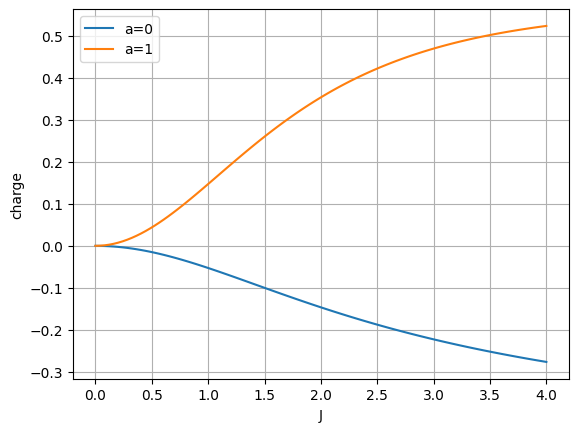
\includegraphics[width=0.45\columnwidth]{plots/numerical/Alice/N1_charge_vs_J.png}
    }
    \hfill
    \subfloat[\( N = 2 \)]{
        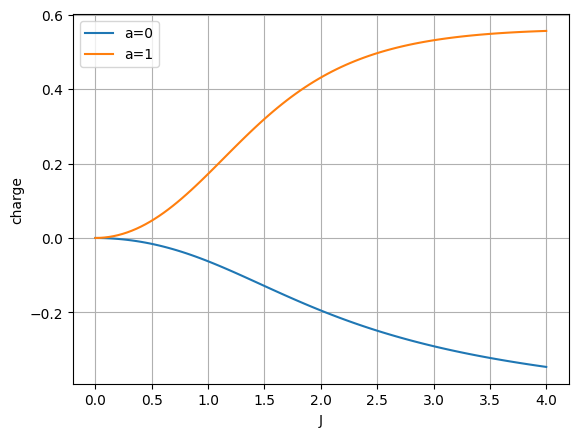
\includegraphics[width=0.45\columnwidth]{plots/numerical/Alice/N2_charge_vs_J.png}
    }

    \medskip
    
    \subfloat[\( N = 3 \)]{
        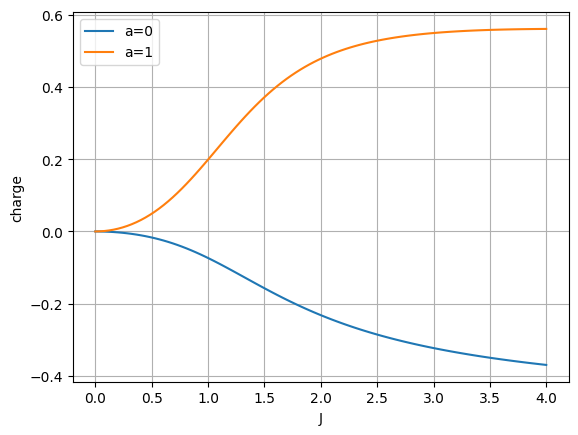
\includegraphics[width=0.45\columnwidth]{plots/numerical/Alice/N3_charge_vs_J.png}
    }
    \hfill
    \subfloat[\( N = 4 \)]{
        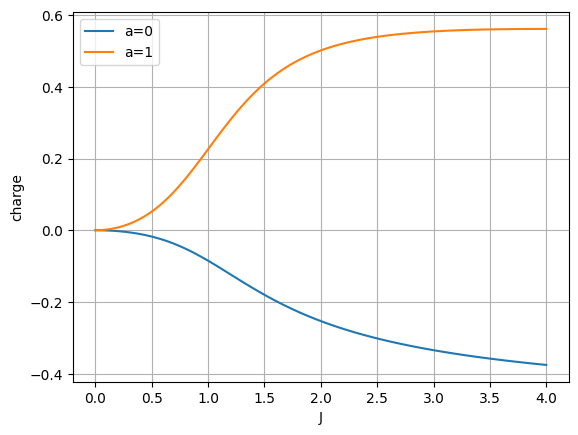
\includegraphics[width=0.45\columnwidth]{plots/numerical/Alice/N4_charge_vs_J.png}
    }
    \caption{\( Q_B \) vs. \( J \), for the star-coupled model \( H^{(1)} \), with \( h=1 \) and \( \sigma_A = X_0 \).}
    \label{fig:alice_x_vs_j}
\end{figure}

\subsubsection{Teleportation Behavior vs Coupling Strength \texorpdfstring{\( J \)}{J}}

Figure~\ref{fig:alice_x_vs_j} shows the simulated expectation values of Bob’s measured observables for the charge protocol, plotted against the interaction strength \( J \). In accordance with theoretical predictions, we observe a clear distinction between the behavior under energy and charge teleportation:
\begin{itemize}
    \item In the \textbf{energy teleportation protocol}, Bob's observable exhibits a nontrivial and asymmetric profile, with maximal negative expectation value at an intermediate value of \( J \), consistent with the optimal teleportation regime identified in Refs.~\cite{IkedaTeleportingCharge, QKDbyQET} (see Appendix Fig.~\ref{fig:alice_vs_hJ} for the full energy data).
    \item In the \textbf{charge teleportation protocol}, the observable expectation values are symmetric and exhibit the expected mirror-image pattern under bit flipping, aligning with the predictions in the teleportation formalism.
\end{itemize}

\subsubsection{Energy vs. Charge Teleportation: Comparative Discussion}

Although energy and charge teleportation protocols share the same structure of local operations and classical communication (LOCC), they differ substantially in their physical implementation and resulting behavior:

\begin{itemize}
    \item \textbf{Energy teleportation} involves local injection and extraction of energy from the entangled ground state. Its effectiveness depends sensitively on the commutation relations between local Hamiltonians, often leading to asymmetric behavior under bit-flip operations. This asymmetry, as seen in our simulations, may pose challenges for extending the protocol to multi-party or long-range quantum networks.
    
    \item \textbf{Charge teleportation}, in contrast, exhibits more symmetric and robust behavior. The observable expectation values at Bob’s site respond linearly and predictably to Alice's bit, enabling straightforward mapping to key bits in QKD. This symmetry not only improves interpretability but also offers resilience to noise and misalignment in measurement bases.
    
    \item \textbf{Scalability of extracted signal—} Importantly, since both energy and charge observables were rescaled to arbitrary units, we may compare their relative magnitudes. Our simulations reveal that the charge expectation value at Bob’s site remains approximately constant as the system size \( N \) increases, whereas the extracted energy diminishes. This suggests that charge teleportation may be more favorable for large-scale implementations, especially in distributed QKD architectures.
    This suggests that charge teleportation may be more favorable for large-scale implementations, especially in distributed QKD architectures. Furthermore, the perfect symmetry of the charge signal is a decisive advantage for cryptography; it ensures that the logical '0' and '1' are equally distinguishable, preventing any potential bias in the raw key that an eavesdropper might exploit.
\end{itemize}

These findings corroborate the observations in~\cite{IkedaTeleportingCharge, QKDbyQET}, where the symmetry and noise robustness of charge-like observables were highlighted. Furthermore, since energy teleportation can depend on subtle inter-site Hamiltonian partitionings (cf. Eq.~(8) in~\cite{QKDbyQET}), it might be less generalizable than charge teleportation for QKD networks involving multiple recipients.

\begin{figure}[ht]
    \centering
    \subfloat[\( N = 2 \), \( \sigma_A = X_0 \)]{
        
\includegraphics[width=0.45\columnwidth]{plots/numerical/NearestNeighbors/X/N2_charge_vs_J.png}
    }
    \hfill
    \subfloat[\( N = 2 \), \( \sigma_A = Y_0 \)]{
        
\includegraphics[width=0.45\columnwidth]{plots/numerical/NearestNeighbors/Y/N2_charge_vs_J.png}
    }

    \medskip

    \subfloat[\( N = 3 \), \( \sigma_A = X_0 \)]{
        
\includegraphics[width=0.45\columnwidth]{plots/numerical/NearestNeighbors/X/N3_charge_vs_J.png}
    }
    \hfill
    \subfloat[\( N = 3 \), \( \sigma_A = Y_0 \)]{
        
\includegraphics[width=0.45\columnwidth]{plots/numerical/NearestNeighbors/Y/N3_charge_vs_J.png}
    }

    \medskip

    \subfloat[\( N = 4 \), \( \sigma_A = X_0 \)]{
        
\includegraphics[width=0.45\columnwidth]{plots/numerical/NearestNeighbors/X/N4_charge_vs_J.png}
    }
    \hfill
    \subfloat[\( N = 4 \), \( \sigma_A = Y_0 \)]{
        
\includegraphics[width=0.45\columnwidth]{plots/numerical/NearestNeighbors/Y/N4_charge_vs_J.png}
    }

    \caption{\( Q_B \) vs. \( J \), for the nearest-neighbors model \( H^{(2)} \), with \( h=1 \).}
    \label{fig:nn_vs_j}
\end{figure}

\subsubsection{Importance of Coupling Ratio and Energy Scale}

As discussed in Section~\ref{sec:alice_hamiltonian}, the essential quantity is the ratio \( h/J \), as the overall energy scale can be rescaled without loss of generality. Therefore, while Fig.~\ref{fig:alice_x_vs_j} presents results as a function of \( J \) with fixed \( h \), the conclusions remain valid under constant ratio rescaling.

Detailed simulations varying \( h \) at fixed \( J \), and the corresponding dependence of teleportation fidelity on field strength, are presented in Appendix~\ref{appendix:numerical-simulation}.

\subsection{Simulation Results: Nearest-Neighbor Hamiltonian}

We now present simulation results for the teleportation protocol under the nearest-neighbor interaction Hamiltonian \( H^{(2)} \), (as defined in equation ~\ref{eq:H2}). Unlike the star-type model, this Hamiltonian restricts Alice’s influence to her immediate neighbor, resulting in significantly reduced and more localized entanglement propagation.

\subsubsection{Protocol Implementation and Basis Choices}

For this interaction pattern, the case \( N = 1 \) is equivalent to the previous star model and is therefore omitted. From \( N = 2 \) and beyond, we simulate both energy and charge teleportation protocols, using two distinct measurement bases for Alice: \( \sigma_A = X \) and \( \sigma_A = Y \).

\subsubsection{Extracted Observables vs. Coupling Strength \texorpdfstring{\( J \)}{J}}

Figure~\ref{fig:nn_vs_j} shows the extracted expectation values at Bob’s site as a function of the coupling \( J \), for both basis choices. As expected, the magnitude of the teleported observable diminishes with increasing system size, reflecting the locality of interaction.

Interestingly, while both energy and charge teleportation degrade as \( N \) increases, the \textbf{energy protocol appears more robust to the choice of measurement basis}. This is clearly seen by the different amplitudes and axis scale in Figure~\ref{fig:nn_vs_j} compared to the energy case.

\subsubsection{Implications for Teleportation Robustness and QKD}

The reduced sensitivity of the energy protocol to the choice of measurement basis is advantageous for realistic applications, especially where full control of Alice’s basis is not guaranteed (e.g., under noise or adversarial disturbances). In contrast, the strong basis-dependence in charge teleportation highlights its utility primarily in well-controlled scenarios.

These findings echo and expand upon the discussion in~\cite{IkedaTeleportingCharge, QKDbyQET}, where energy teleportation was shown to tolerate less structured measurement randomness while still extracting meaningful energy. Our simulations validate this robustness in larger systems with nearest-neighbor coupling.
